\documentclass[12pt,a4paper]{article}

%\usepackage[left=1.5cm,right=1.5cm,top=1cm,bottom=2cm]{geometry}
\usepackage[in, plain]{fullpage}
\usepackage{array}
\usepackage{../../../pas-math}
\usepackage{../../../moncours}


%\usepackage{pas-cours}
%-------------------------------------------------------------------------------
%          -Packages nécessaires pour écrire en Français et en UTF8-
%-------------------------------------------------------------------------------
\usepackage[utf8]{inputenc}
\usepackage[frenchb]{babel}
\usepackage[T1]{fontenc}
\usepackage{lmodern}
\usepackage{textcomp}



%-------------------------------------------------------------------------------

%-------------------------------------------------------------------------------
%                          -Outils de mise en forme-
%-------------------------------------------------------------------------------
\usepackage{hyperref}
\hypersetup{pdfstartview=XYZ}
%\usepackage{enumerate}
\usepackage{graphicx}
\usepackage{multicol}
\usepackage{tabularx}
\usepackage{multirow}


\usepackage{anysize} %%pour pouvoir mettre les marges qu'on veut
%\marginsize{2.5cm}{2.5cm}{2.5cm}{2.5cm}

\usepackage{indentfirst} %%pour que les premier paragraphes soient aussi indentés
\usepackage{verbatim}
\usepackage{enumitem}
\usepackage[usenames,dvipsnames,svgnames,table]{xcolor}

\usepackage{variations}

%-------------------------------------------------------------------------------


%-------------------------------------------------------------------------------
%                  -Nécessaires pour écrire des mathématiques-
%-------------------------------------------------------------------------------
\usepackage{amsfonts}
\usepackage{amssymb}
\usepackage{amsmath}
\usepackage{amsthm}
\usepackage{tikz}
\usepackage{xlop}
%-------------------------------------------------------------------------------



%-------------------------------------------------------------------------------


%-------------------------------------------------------------------------------
%                    - Mise en forme avancée
%-------------------------------------------------------------------------------

\usepackage{ifthen}
\usepackage{ifmtarg}


\newcommand{\ifTrue}[2]{\ifthenelse{\equal{#1}{true}}{#2}{$\qquad \qquad$}}

%-------------------------------------------------------------------------------

%-------------------------------------------------------------------------------
%                     -Mise en forme d'exercices-
%-------------------------------------------------------------------------------
%\newtheoremstyle{exostyle}
%{\topsep}% espace avant
%{\topsep}% espace apres
%{}% Police utilisee par le style de thm
%{}% Indentation (vide = aucune, \parindent = indentation paragraphe)
%{\bfseries}% Police du titre de thm
%{.}% Signe de ponctuation apres le titre du thm
%{ }% Espace apres le titre du thm (\newline = linebreak)
%{\thmname{#1}\thmnumber{ #2}\thmnote{. \normalfont{\textit{#3}}}}% composants du titre du thm : \thmname = nom du thm, \thmnumber = numéro du thm, \thmnote = sous-titre du thm

%\theoremstyle{exostyle}
%\newtheorem{exercice}{Exercice}
%
%\newenvironment{questions}{
%\begin{enumerate}[\hspace{12pt}\bfseries\itshape a.]}{\end{enumerate}
%} %mettre un 1 à la place du a si on veut des numéros au lieu de lettres pour les questions 
%-------------------------------------------------------------------------------

%-------------------------------------------------------------------------------
%                    - Mise en forme de tableaux -
%-------------------------------------------------------------------------------

\renewcommand{\arraystretch}{1.7}

\setlength{\tabcolsep}{1.2cm}

%-------------------------------------------------------------------------------



%-------------------------------------------------------------------------------
%                    - Racourcis d'écriture -
%-------------------------------------------------------------------------------

% Angles orientés (couples de vecteurs)
\newcommand{\aopp}[2]{(\vec{#1}, \vec{#2})} %Les deuc vecteurs sont positifs
\newcommand{\aopn}[2]{(\vec{#1}, -\vec{#2})} %Le second vecteur est négatif
\newcommand{\aonp}[2]{(-\vec{#1}, \vec{#2})} %Le premier vecteur est négatif
\newcommand{\aonn}[2]{(-\vec{#1}, -\vec{#2})} %Les deux vecteurs sont négatifs

%Ensembles mathématiques
\newcommand{\naturels}{\mathbb{N}} %Nombres naturels
\newcommand{\relatifs}{\mathbb{Z}} %Nombres relatifs
\newcommand{\rationnels}{\mathbb{Q}} %Nombres rationnels
\newcommand{\reels}{\mathbb{R}} %Nombres réels
\newcommand{\complexes}{\mathbb{C}} %Nombres complexes


%Intégration des parenthèses aux cosinus
\newcommand{\cosP}[1]{\cos\left(#1\right)}
\newcommand{\sinP}[1]{\sin\left(#1\right)}


%Probas stats
\newcommand{\stat}{statistique}
\newcommand{\stats}{statistiques}
%-------------------------------------------------------------------------------

%-------------------------------------------------------------------------------
%                    - Mise en page -
%-------------------------------------------------------------------------------

\newcommand{\twoCol}[1]{\begin{multicols}{2}#1\end{multicols}}


\setenumerate[1]{font=\bfseries,label=\textit{\alph*})}
\setenumerate[2]{font=\bfseries,label=\arabic*)}


%-------------------------------------------------------------------------------
%                    - Elements cours -
%-------------------------------------------------------------------------------






\date{}
\title{}


\begin{document}
%\maketitle
\chap[num=5, color=red]{Exponentielles et logarithme décimal}{Olivier FINOT, \today }

\section{Fonction exponentielle de base $q$}

\subsection{Définition}
\begin{mydef}
	 $q$ est un nombre strictement positif ($q > 0$).
	 La fonction qui à tout nombre $x$ associe $q^x$, est appelée \kw{fonction exponentielle} de base $q$.
\end{mydef}

\begin{myex}
	\begin{itemize}
		\item La fonction $f$, définie par $f(x)=2^x$, est la \kw{fonction exponentielle de base $2$}. 
		\item La fonction $g$, définie par $g(x)=0,5^x$, est la \kw{fonction exponentielle de base $0,5$}.
	\end{itemize}
	
\end{myex}


\subsection{Valeurs particulières et variations}

\begin{myprops}
	\begin{enumerate}
		\item Valeurs particulières :
		
		\begin{center}
			\begin{align*}
				q^0 = 1 \qquad\qquad\qquad\qquad\qquad q^1 = q 			
			\end{align*}
		\end{center}
		
		
		\item Variations :
			\begin{itemize}
				\item Si \kw{$q > 0$}, alors la fonction est \kw{croissante}.
				\item Si \kw{$q < 0$}, alors la fonction est \kw{décroissante}.
			\end{itemize}
	\end{enumerate}
\end{myprops}

\begin{myex}
	\begin{multicols}{2}
		$f(x)= 2^x$, $2 > 1$\\
		la fonction $f$ est croissante
		
		\begin{center}
			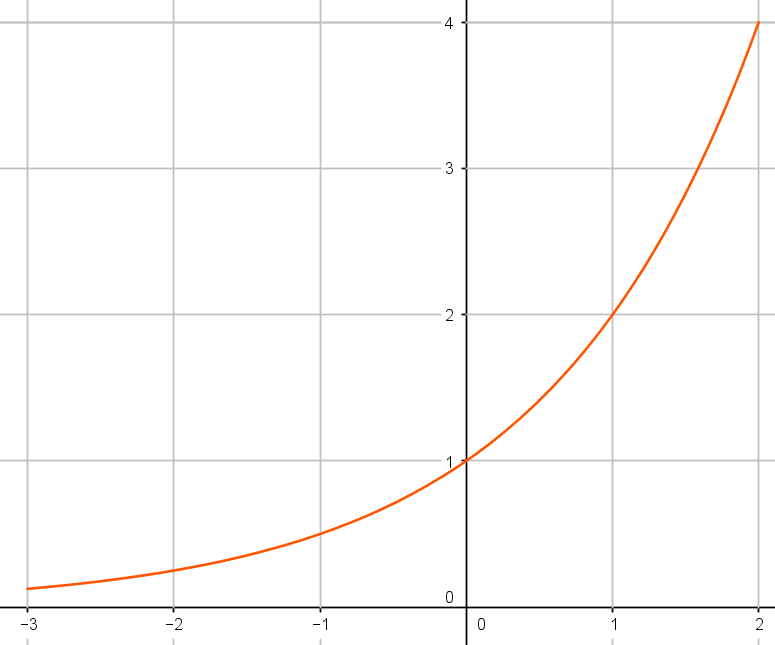
\includegraphics[scale=0.3]{./img/var1}
		\end{center}
		
		\ \\
		$g(x)= 0,5^x$, $0,5 > 1$\\
		la fonction $g$ est décroissante
		
		\begin{center}
			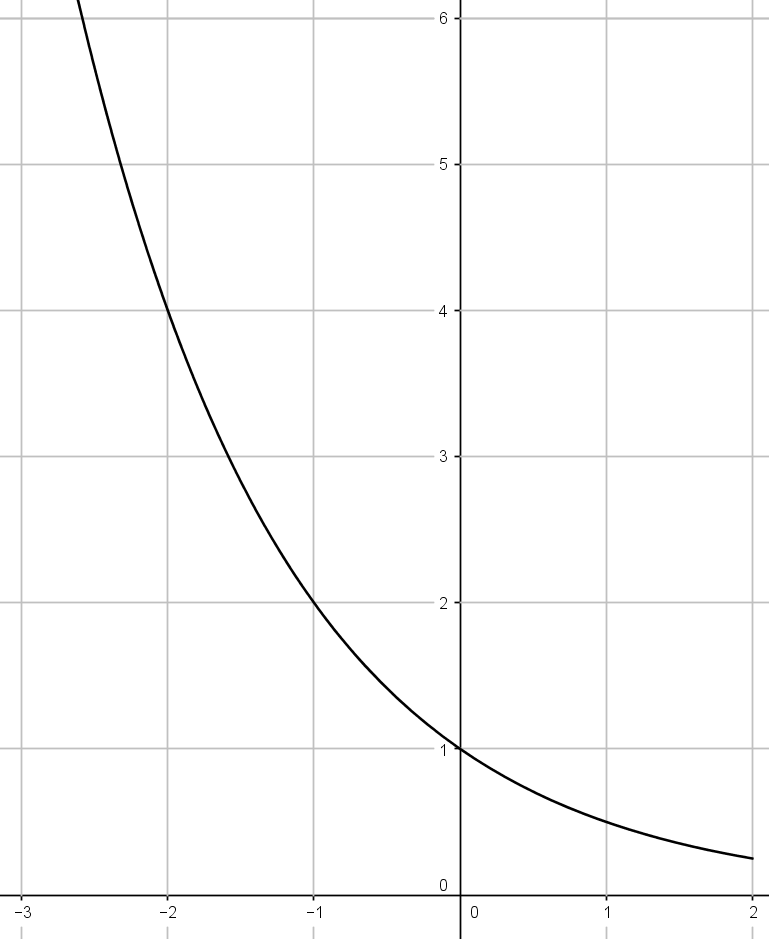
\includegraphics[scale=0.25]{./img/var2}
		\end{center}
	\end{multicols}
\end{myex}

\subsection{Règles de calcul}

\begin{myprops}
	Les règles de calculs sont les mêmes que pour les puissances entières.\\
	$a$ et $b$ sont deux nombres quelconques et $q$ un nombre strictement positif.
	
	\begin{align*}
		q^a = q^b &\Leftrightarrow a = b\\
		q^x \times q^y &= q^{a+b}\\
		\frac{q^a}{q^b} &= q^{a-b}\\
		(q^a)^b &= q^{a \times b}
	\end{align*}
\end{myprops}

\begin{myex}
	
	\begin{align*}
		2^{-4} \times 2^{1,5} &= 2^{-2,5}\\
		\frac{0,1^3}{0,1^{1,8}} &= 0,1^{1,2}\\
		(3^{0,4})^{-2} &= 3^{-0,8}
	\end{align*}
\end{myex}

\newpage

\section{Fonction logarithme décimal}

\subsection{Définition}

\begin{mydef}
	$a$ est un nombre strictement positif ($a>0$), le nombre $b$ tel que \kw{$10^b=a$}, est le \kw{logarithme décimal}, noté $\log a$.
\end{mydef}

\subsection{Valeurs particulières et variations}

\begin{myprops}
	\begin{enumerate}
		\item Valeurs particulières :
			\begin{align*}
				\log 1 &= 0 \\
				\log 10 &= 1\\
				\log 100 &= 2
			\end{align*}
	
		\item Signe et variations :
			La fonction $\log x$ est \kw{croissante} pour $x > 0$.
			
			 Si $0 \leq x < 1$, alors $\log x$ est négatif.
			 
			 Si $x \geq 1$, alors $\log x$ est positif.
			\begin{center}
				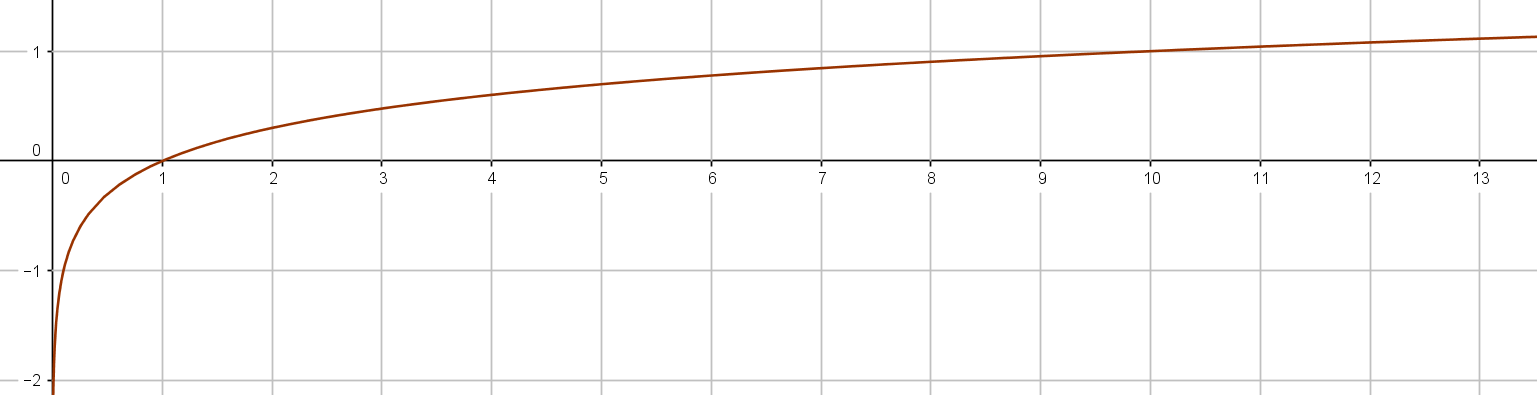
\includegraphics[scale = 0.35]{./img/var_log}
			\end{center}	
	\end{enumerate}
	
	
\end{myprops}

\subsection{Règles de calcul}

\begin{myprops}
	$a$ et $b$ sont deux nombres strictement positifs :
	
	\begin{align*}
		\log a = b &\Leftrightarrow a = 10^b \\
		10^b = a &\Leftrightarrow b = \log a \\
		\log a = \log b &\Leftrightarrow a = b \\
		\log a < \log b &\Leftrightarrow a < b \\
		\log (a \times b) &= \log a + \log b \\
		\log  \left( \frac{a}{b} \right) &= \log a - \log b \\
		\log(a^x) &= x \times log a 
	\end{align*}
\end{myprops}
\end{document}